\DAsection[分支负责隔离，Pull Request 负责让变化被看见、被讨论、被批准]{GitHub 团队协作工作流}

\begin{frame}{3.1 两种常见协作模型}{同仓库分支适合内部团队，Fork 适合外部贡献}
  \begin{columns}[T]
    \begin{column}{0.48\textwidth}
      \begin{block}{Shared Repository}
        \begin{itemize}
          \item 成员对同一仓库有写权限
          \item 每人创建 Topic Branch
          \item PR 合并回 \DAfile{main}
          \item 适合课程小组、公司内部项目
        \end{itemize}
      \end{block}
    \end{column}
    \begin{column}{0.48\textwidth}
      \begin{block}{Fork + Pull Request}
        \begin{itemize}
          \item 贡献者在自己的 Fork 中修改
          \item 向上游仓库发起 PR
          \item 通过 Fork 向上游提交变更
          \item 适合开源、外部合作方
        \end{itemize}
      \end{block}
    \end{column}
  \end{columns}
  \DAtagline{课程选择}{优先使用 Shared Repository，减少初学阶段的 remote / upstream 复杂度}
\end{frame}

\begin{frame}{3.2 从需求到代码：先拆任务，再建分支}{一个分支对应一个独立工作单元}
  \centering
  \begin{tikzpicture}[node distance=2mm]
    \node[DAflow,minimum width=18mm] (issue) {Issue\\定义问题};
    \node[DAflow,minimum width=18mm,right=of issue] (owner) {Assign\\负责人};
    \node[DAflow,minimum width=18mm,right=of owner] (branch) {Branch\\隔离};
    \node[DAflow,minimum width=18mm,right=of branch] (commit) {Commit\\记录};
    \node[DAflow,minimum width=18mm,right=of commit] (pr) {PR\\审查};
    \node[DAflow,minimum width=18mm,right=of pr] (done) {Merge\\完成};
    \draw[DAarrowred] (issue) -- (owner);
    \draw[DAarrowred] (owner) -- (branch);
    \draw[DAarrowred] (branch) -- (commit);
    \draw[DAarrowred] (commit) -- (pr);
    \draw[DAarrowred] (pr) -- (done);
  \end{tikzpicture}
  \par\medskip
  \begin{itemize}
    \item Issue 写清背景、范围、完成条件与边界。
    \item 分支名带任务语义；PR 描述中关联 Issue。
    \item 一个分支只服务一个目标，减少冲突与 Review 负担。
  \end{itemize}
\end{frame}

\begin{frame}[fragile]{3.3 开发者的完整命令流}{同步、建分支、提交、推送}
  \begin{lstlisting}[language=bash]
git switch main
git pull --ff-only
git switch -c feature/chat-history

# edit and test
git status
git diff
git add src/
git commit -m "feat(chat): load conversation history"

git push -u origin feature/chat-history
  \end{lstlisting}
  \DAtagline{关键动作}{首次 push 后立即创建 Pull Request}
\end{frame}

\begin{frame}{3.4 Pull Request：提交变更提案}{base 是要进入的分支，compare 是你的分支}
  \centering
  \DAframed{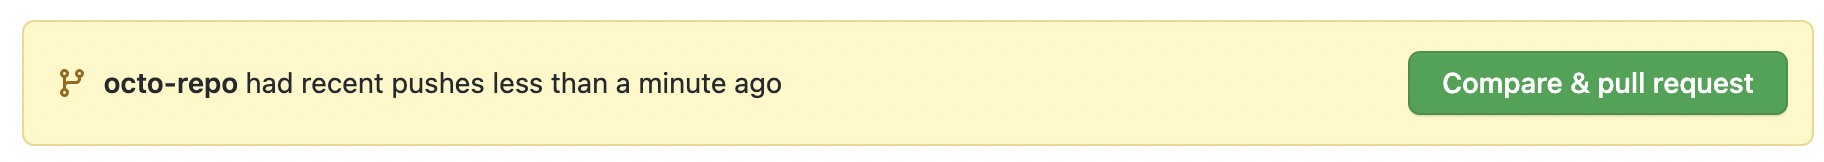
\includegraphics[width=111mm]{assets/official/github-compare-pr.png}}
  \begin{itemize}
    \item 标题说明结果，正文解释背景、方案、测试证据与风险。
    \item Draft PR 可尽早暴露方向，避免做完才发现设计不对。
    \item PR 后续新增 Commit 会自动进入同一个审查上下文。
  \end{itemize}
  \DAsource{GitHub Docs · Creating a pull request}{https://docs.github.com/en/pull-requests/collaborating-with-pull-requests/proposing-changes-to-your-work-with-pull-requests/creating-a-pull-request}
\end{frame}

\begin{frame}{3.5 一个合格 PR 描述应该包含什么}{让 Review 者快速理解}
  \begin{columns}[T]
    \begin{column}{0.48\textwidth}
      \begin{block}{建议模板}
        \begin{itemize}
          \item \textbf{Why}：为什么要改
          \item \textbf{What}：核心改动
          \item \textbf{How to test}：如何验证
          \item \textbf{Screenshots}：界面证据
          \item \textbf{Risk / rollback}：风险与回滚
        \end{itemize}
      \end{block}
    \end{column}
    \begin{column}{0.48\textwidth}
      \begin{alertblock}{避免}
        \begin{itemize}
          \item “改好了，请看”
          \item 没有说明数据库迁移
          \item 没有列环境变量变化
          \item 把多个不相关任务塞进一个 PR
          \item 自己都没打开 Files changed
        \end{itemize}
      \end{alertblock}
    \end{column}
  \end{columns}
\end{frame}

\begin{frame}{3.6 Code Review 看什么}{先看正确性和风险，再看风格}
  \centering
  \DAframed{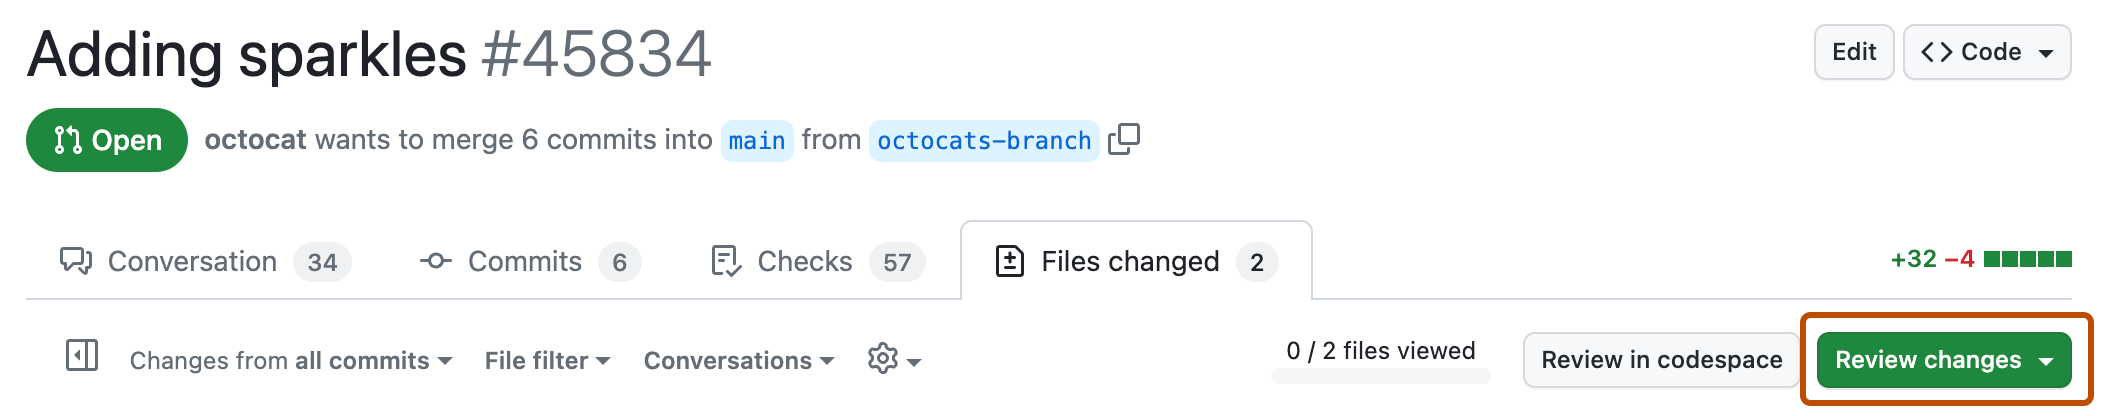
\includegraphics[width=119mm]{assets/official/github-review-changes.png}}
  \begin{itemize}
    \item 需求是否真的满足？边界条件、错误处理、权限校验是否完整？
    \item 是否引入密钥、调试代码、重复逻辑或破坏兼容性？
    \item Review 结论：Comment、Approve、Request changes。
  \end{itemize}
  \DAsource{GitHub Docs · Reviewing proposed changes}{https://docs.github.com/en/pull-requests/collaborating-with-pull-requests/reviewing-changes-in-pull-requests/reviewing-proposed-changes-in-a-pull-request}
\end{frame}

\begin{frame}{3.7 Review 评论要对事、可执行}{指出风险，也给出下一步}
  \begin{DAtable}{@{}p{34mm}p{83mm}@{}}
    \toprule
    评论类型 & 示例 \\
    \midrule
    阻塞问题 & 这里把用户 ID 直接相信前端传值，会产生越权，请从 Token 读取身份。 \\
    建议改进 & 建议把重复的请求逻辑提取到 API Client；本 PR 不阻塞，可另开任务。 \\
    澄清问题 & 这里为何选择 204？前端是否读取响应正文？ \\
    肯定反馈 & 这个错误结构与现有接口一致，前端处理会更简单。 \\
    \bottomrule
  \end{DAtable}
  \DAtagline{团队文化}{Review 代码，不评价人；问题要具体到行为、风险与验证方式}
\end{frame}

\begin{frame}{3.8 三种合并方式怎么选}{小团队建议默认 Squash merge}
  \begin{DAtable}{@{}p{28mm}p{43mm}p{48mm}@{}}
    \toprule
    方式 & 历史结果 & 适用场景 \\
    \midrule
    Merge commit & 保留分支与所有 Commit & 需要完整分支拓扑 \\
    Squash merge & PR 压成一个 Commit & 功能分支过程较碎，小团队默认 \\
    Rebase merge & 每个 Commit 线性接到 main & Commit 本身质量高、团队熟悉 Rebase \\
    \bottomrule
  \end{DAtable}
  \begin{itemize}
    \item 规则要统一，否则历史一会儿分叉、一会儿线性，回滚与排查更难。
    \item Squash 后 PR 标题应成为高质量 Commit 信息。
  \end{itemize}
\end{frame}

\begin{frame}[fragile]{3.9 PR 开发期间如何同步 main}{降低最终合并时的冲突}
  \begin{columns}[T]
    \begin{column}{0.48\textwidth}
      \begin{block}{Merge main}
        \begin{lstlisting}[language=bash]
git fetch origin
git switch feature/chat-history
git merge origin/main
        \end{lstlisting}
        \scriptsize 保留真实分叉关系，不重写已有 Commit。
      \end{block}
    \end{column}
    \begin{column}{0.48\textwidth}
      \begin{block}{Rebase onto main}
        \begin{lstlisting}[language=bash]
git fetch origin
git switch feature/chat-history
git rebase origin/main
        \end{lstlisting}
        \scriptsize 历史更线性，但会重写分支 Commit ID。
      \end{block}
    \end{column}
  \end{columns}
  \DAtagline{约定}{初学团队优先 Merge；熟悉 Rebase 后由团队统一切换}
\end{frame}

\begin{frame}{3.10 密钥必须留在 Git 之外}{泄漏后立即轮换并清理历史}
  \begin{alertblock}{严禁提交}
    \DAfile{.env}、数据库密码、JWT Secret、云厂商密钥、模型 API Key、私钥文件。
  \end{alertblock}
  \begin{itemize}
    \item 发现泄漏后立即吊销或轮换密钥，再处理仓库文件。
    \item 再清理 Git 历史、检查 Fork / 缓存 / CI 日志，并复盘为何未被拦截。
    \item 部署时通过服务器环境变量、Secret 文件或平台 Secret 注入。
  \end{itemize}
  \DAtagline{提交前检查}{\DAcmd{git diff --staged} + Secret Scanner + 最小权限密钥}
\end{frame}
